%%%%%%%%%%%%%%%%%%%%%%%%%%%%%%%%%%%%%%%%%%%%%%%%%%%%%%%
%% Engineer & Master Thesis, LaTeX Template          %%
%% Copyleft by Piotr Woźniak & Artur M. Brodzki      %%
%% Faculty of Electronics and Information Technology %%
%% Warsaw University of Technology, Warsaw, 2019     %%
%%%%%%%%%%%%%%%%%%%%%%%%%%%%%%%%%%%%%%%%%%%%%%%%%%%%%%%

\documentclass[
    left=2.5cm,         % Sadly, generic margin parameter
    right=2.5cm,        % doesnt't work, as it is
    top=2.5cm,          % superseded by more specific
    bottom=3cm,         % left...bottom parameters.
    bindingoffset=6mm,  % Optional binding offset.
    nohyphenation=true % You may turn off hyphenation, if don't like. =false
]{eiti/eiti-thesis} % bazuje na clasie mwart

\nocite{*}

\usepackage[
    backend=bibtex,
]{biblatex}
\usepackage{csquotes}
\usepackage{hyperref}
\usepackage{algpseudocode}
\usepackage{algorithm}
\usepackage{url}

\langpol % Dla języka angielskiego mamy \langeng
\graphicspath{{img/}}             % Katalog z obrazkami.
\bibliography{bib-mendeley.bib,bib-other.bib} % Plik .bib z bibliografią`'

\makeatletter
\xpatchcmd\lst@MakeCaption{\protect\numberline{\thelstlisting}\lst@@caption}{\protect\numberline{\thelstlisting.}\lst@@caption}{}{}
%\makeatother
%\makeatletter
%\xpatchcmd{\LT@c@ption}{\protect\numberline{\thetable}}{\protect\numberline.{. \thetable . }}{}{}
\makeatother

\begin{document}

%--------------------------------------
% Strona tytułowa
%--------------------------------------
\RaportThesis
\instytut{Cyberbezpieczeństwa}
\kierunek{Telekomunikacja}
\specjalnosc{Techniki Teleinformatyczne}
\title{
    Akceleracja sprzętowa kryptoanalizy algorytmów kryptograficznych
}
\engtitle{ % Tytuł po angielsku do angielskiego streszczenia
    Hardware acceleration of cryptoanalysis of cryptograhpic algorithms
}
\author{Andrzej Tłomak}
\album{311450}
\promotor{dr. hab. inż. Mariusz Rawski}
\date{\the\year}
\maketitle

%--------------------------------------
% Streszczenie po polsku
%--------------------------------------
\streszczenie
Cel pracy
\slowakluczowe Krzywe eliptyczne, Kryptografia, Kryptoanaliza, CUDA, Algorytm~rho~Pollard'a

\newpage

%--------------------------------------
% Streszczenie po angielsku
%--------------------------------------
\abstract
The objective of this phase included a review of the literature describing the current State-of-Art \
in cryptoanalysis of systems \
based on Elliptic curves in Finite Fields. It involved getting deeper knowledge of theory
and mathematical fundation of Elliptic curves as well as setting up an environment
to develop implementation utillizing CUDA technology.
\keywords Elliptic curves, Cryptography, Cryptoanalysis, CUDA, FPGA, rho~Pollard~algorithm
\newpage

%--------------------------------------
% Oświadczenie o autorstwie
%--------------------------------------
\makeauthorship
\blankpage

%--------------------------------------
% Spis treści
%--------------------------------------
%\thispagestyle{empty}
\tableofcontents
%\blankpage

%--------------------------------------
% Rozdziały
%--------------------------------------
\newpage
\section{Wprowadzenie}
Celem tej pracy była implementacja akecleracji sprzętowej algorytmu do kryptoanalizy kryptosystemów opartych
o problem logarytmu dyskretnego. Jednym z prostszych sposobów akceleracji algorytmów które
pozwalają na ich zrównoleglenie, jest wykorzystanie procesorów graficznych GPGPU.
Praca ta skupia się na wykorzystaniu framework'u Nvidia CUDA wraz z kartą graficzną Nvidia GTX 2070 Super
do przyśpieszenia kryptoanalizy krzywej ECCp-79 z listy Certicom.

\newpage % Zaleca się otwieranie rozdziału od nowej strony.
\section{Wstęp teoretyczny}
\subsection{Ciało skończone}
Ciało skończone jest to ciało ze skończoną liczbą elementów.
Aby ciało spełniało wszystkie założenia, musi ono być rzędu
{\textit p} gdzie {\textit p} jest liczbą pierwszą. Dopuszczalne są również ciała
rzędu \(p^n\) gdzie {\textit p} to liczba pierwsza oraz \( n \geqslant 1\).
W zastosowaniach kryptograficznych, często stosowanym ciałem jest tzw. ciało binarne
postaci \(\mathbb{F}_{2^n}\).
Challange ECC Certicom dopuszcza rozwiązania zarówno na ciele binarnym jak
i ciele rzędu liczba pierwsza.
W swojej pracy skupiłem się wyłącznie na ciałach rzędu {\textit p} liczba pierwsza.

\subsection{Grupa}
% TODO dodać więcej info


\subsection{Problem logarytmu dyskretnego}
Problem logarytmu dyskretnego (\textbf{DLP}) jest
podstawą wielu kryptosystemów.
Jednymi z bardziej znanych są kryptosystem ElGamala oraz protokół wymiany
kluczy Diffie-Hellmana'a.
\\ Problem logarytmu dyskretnego można zdefiniować na grupach cyklicznych.
zarówno na grupie multiplikatywnej $(\mathbb{G},\cdot)$
oraz grupie addytywnej $(\mathbb{G}, +)$, przy odpowiednim zdefiniowaniu działań grupowych.

% TODO spytać czy można definicje 1 - 1 z ksiązki??
\begin{definition}
    Jeżeli G jest grupą cykliczną a $\gamma$ jej generatorem, to logarytmem dyskretnym
    elementu $\alpha \in G$ nazywamy najmniejszą nieujemną liczbę całkowitą x taką, że:
    \[x = \log_{\gamma}{\alpha}\]
\end{definition}
operacji dodawania na krzywej eliptycznej $(\mathbb{E},+)$ \cite{stinson21}.
% 
\subsection{DLP w grupie multiplikatywnej}
Jeżeli $\mathbb{G}$ to (skończona) grupa multiplikatywna, $\alpha \in \mathbb{G}$
to element rzędu $n$ oraz $\beta \in \mathbb{<\alpha>}$ (jest w podgrupie generowanej
przez $\alpha$), to uważane za problematyczne jest znalezienie takiej liczby $a$:
\[a \in \mathbb{Z} \textrm{ oraz } 0\le a \le n-1\]
że:
\[\alpha ^ a = \beta\]
% 
Liczbę $a$ można przedstawić jako:
\[\log_{\alpha}{\beta}\]
% 
% 
\subsection{DLP w grupie addytywnej}
W przypadku krypografii opartej o krzywe eliptyczne, DLP dotyczy
grupy addytywnej $(\mathbb{E},+)$ zdefiniowanej na krzywej eliptycznej.
Niech $\alpha$ jest rzędu n.
W takim przypadku, ponieważ operacją na grupie jest dodawanie modulo n, to działanie
potęgowania przedstawia się jako:
\[\alpha \cdot a = \beta \textrm{ (mod } n)\]
Przy odpowiednim wyborze grupy addytywnej, rozwiązanie problemu logarytmu dyskretnego,
tj. znalezienie $a$,
jest trudne \cite{chrzaszczyk2010}\cite{stinson21}.
\subsection{Krzywe eliptyczne}
Krzywą eliptyczną nieosobliwą nad ciałem $\mathbb{K}$ o charakterystyce różnej od 2 i 3 definiuje się
za jako zbiór rozwiązań $(x,y) \in \mathbb{R} \times \mathbb{R}$ równiania: \cite*{stinson21}
\[y^2 = x^3 + ax + b\]
przy założeniu, że stałe $a, b$ takie, że:
\[4a^3 + 27b^2 \not= 0\]
Jest to tak zwana forma {\textit Weierstrassa} krzywej eliptycznej.
% 
\subsubsection{Krzywe eliptyczne na liczbach rzeczywistych}
% 
Krzywe eliptyczne zdefiniowane na liczbach rzeczywistych nie są kluczowe w
systemach kryptograficznych\cite*{chrzaszczyk2010}\cite*{stinson21}, ale takie ustawienia
pozwalają na prostsze przedstawienie niektórych zagadnień
np. dodawnie punktów na krzywej.
\begin{figure}[!h]
    \centering 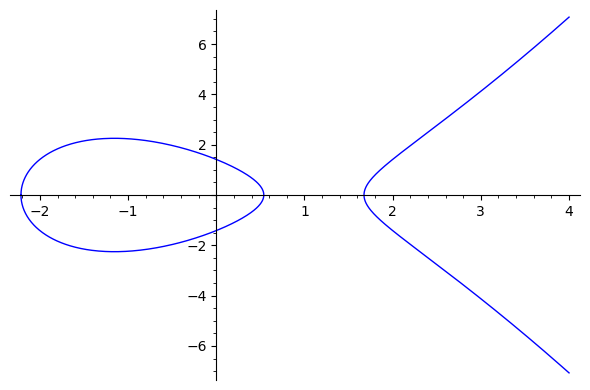
\includegraphics[width=0.8\linewidth]{sage/krzywa_-4_2.png}
    \caption{Krzywa eliptyczna $y^2=x^3-4+2$}
\end{figure}
% 
\subsubsection*{Krzywe eliptyczne na ciele skończonym}
Krzywa eliptyczna na ciele skończonym jest stosowana w kryptografii.
Z powodu charakterystyki ciała, jej wykres
nie przypomina krzywej na liczbach rzeczywistych.
Krzywa taka składa się z punktów, których współrzędne należą do ciała
na którym jest opisana.
Wszystkie operacje na krzywej, takie jak dodawanie, wykonuje się
również z zastosowaniem operacji modulo rzędu ciała.
\begin{figure}[!h]
    \centering 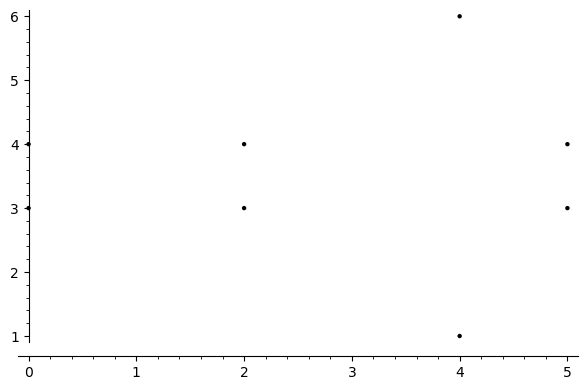
\includegraphics[width=0.8\linewidth]{sage/elliptic_finite_field.png}
    \caption{Krzywa eliptyczna $y^2=x^3-4+2$ nad $GF(7)$}
\end{figure}
% 
\subsubsection{Dodawanie punktów na krzywej eliptycznej}
Przedstwienie krzywej eliptycznej na ciele liczb rzeczywistych,
umożliwia proste zwizualizowanie geometrycznej interpretacji dodawania punktów
leżących na krzywej.
\newline
\indent
Geometryczne dodawanie punktów na krzywej eliptycznej polega na połączeniu
dwóch punktów $P$ i $Q$ prostopadłą linią, która przecina krzywą w trzecim
punkcie, $R'$. Następnie, wynikowy punkt $R$, będący sumą $P+QP+Q$, znajdujemy przez
odbicie punktu $R'$ względem osi $x$. W przypadku dublowania punktu, czyli dodawania
punktu PP do siebie samego, rysujemy styczną do krzywej w punkcie $P$, która przecina
krzywą w nowym punkcie. Odbicie tego punktu względem osi $x$ daje nam wynik $2P$.
\newline
Kod w SageMath użyty do wizualizacji dodawania: listing \ref*{sage_1}
\begin{figure}[!h]
    \centering 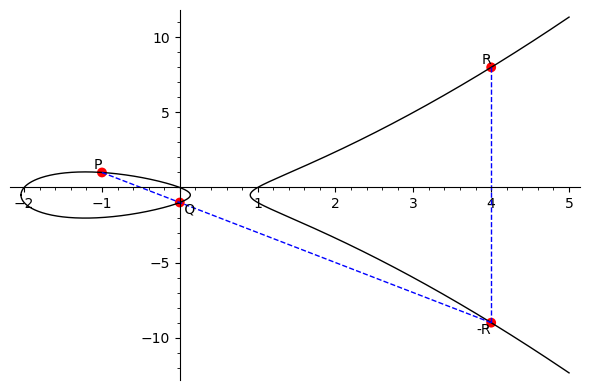
\includegraphics[width=0.8\linewidth]{sage/elliptic_rational_point_addition.png}
    \caption{P + Q na krzywej eliptycznej $y^2+y=x^3-x^2+2x$}
\end{figure}
\newpage
% 
\subsubsection{Dodawanie punktów na krzywej zdefiniowanej na ciele skończonym}
Dodawanie punktów krzywej eliptycznej na ciele skończonym nie ma przejrzyjstej
reprezentacji geometrycznej.
W tym celu stosuje się podejście analityczne.
Wtedy, dodawanie wygląda w następujący sposób:
\begin{enumerate}
    \item Przypadek, gdy \( P \neq Q \):
    \begin{align}
        \lambda & = \frac{y_2 - y_1}{x_2 - x_1}, \\
        x_3     & = \lambda^2 - x_1 - x_2,       \\
        y_3     & = \lambda(x_1 - x_3) - y_1
    \end{align}
    \item Przypadek, gdy \( P = Q \):
    \begin{align*}
        \lambda & = \frac{3x_1^2 + a}{2y_1}, \\
        x_3     & = \lambda^2 - 2x_1,        \\
        y_3     & = \lambda(x_1 - x_3) - y_1
    \end{align*}
\end{enumerate}
Dodawanie punktów w SageMath listing \ref{sage_1}


\section{Koncepcja}
Projekt zakłada zaimplemntowanie systemu do obliczania logarytmu dyskretnego na krzywej eliptycznej.
W celu akceleracji obliczeń wykorzystuje koprocesor jakim jest GPU. Ponieważ równoległy algorytm Rho Pollarda
zakłada architekturę w postaci klient-serwer, to na projekt składa się program pełniący rolę centralnego serwera,
oraz program kliencki wykonujący obliczenia na GPU, uruchamiany w wielu instancjach.
\par
Zarówno program serwera jak i klienta, działają w ramach jednego PC, jednak architektura pozwala na wykorzystanie
wiecej niż jednej karty graficznej w celu przyspieszenia obliczeń.
Program serwera jest zaimplementowany z wykorzystaniem języka Python i odpowiada za gromadzenie znalezionych
punktów oraz za generację nowych punktów startowych. W celu optymalnego przechowywania punktów, wykorzystuje
hash mapę w formie: (\textit{współrzędne punktu} : \textit{seed}), która pozwala na szybkie sprawdzanie czy dany punkt już został znaleziony,
oraz porównanie ziarna użytego do wygenerowania punktu początkowego.
\par
Część klienta odpowiedzialna za komunikację z serwerem,
również jest zaimplementowana w języku Python i za pomocą interfejsu ABI zleca obliczenia do programu napisanego z wykorzystaniem
CUDA C++. Zarówno program serwera jak i każdego z działających klientów, uruchamiany jest w osobnym wątku, co pozwala współbieżne szukanie kolizji i efektywne
kolejkowanie kolejnych serii obliczeń na GPU.
\par
W celu komunikacji klientów z serwerem, wykorzystywane są asynchroniczne kolejki z biblioteki standardowej Pythona.
\begin{figure}[!h]
    \centering 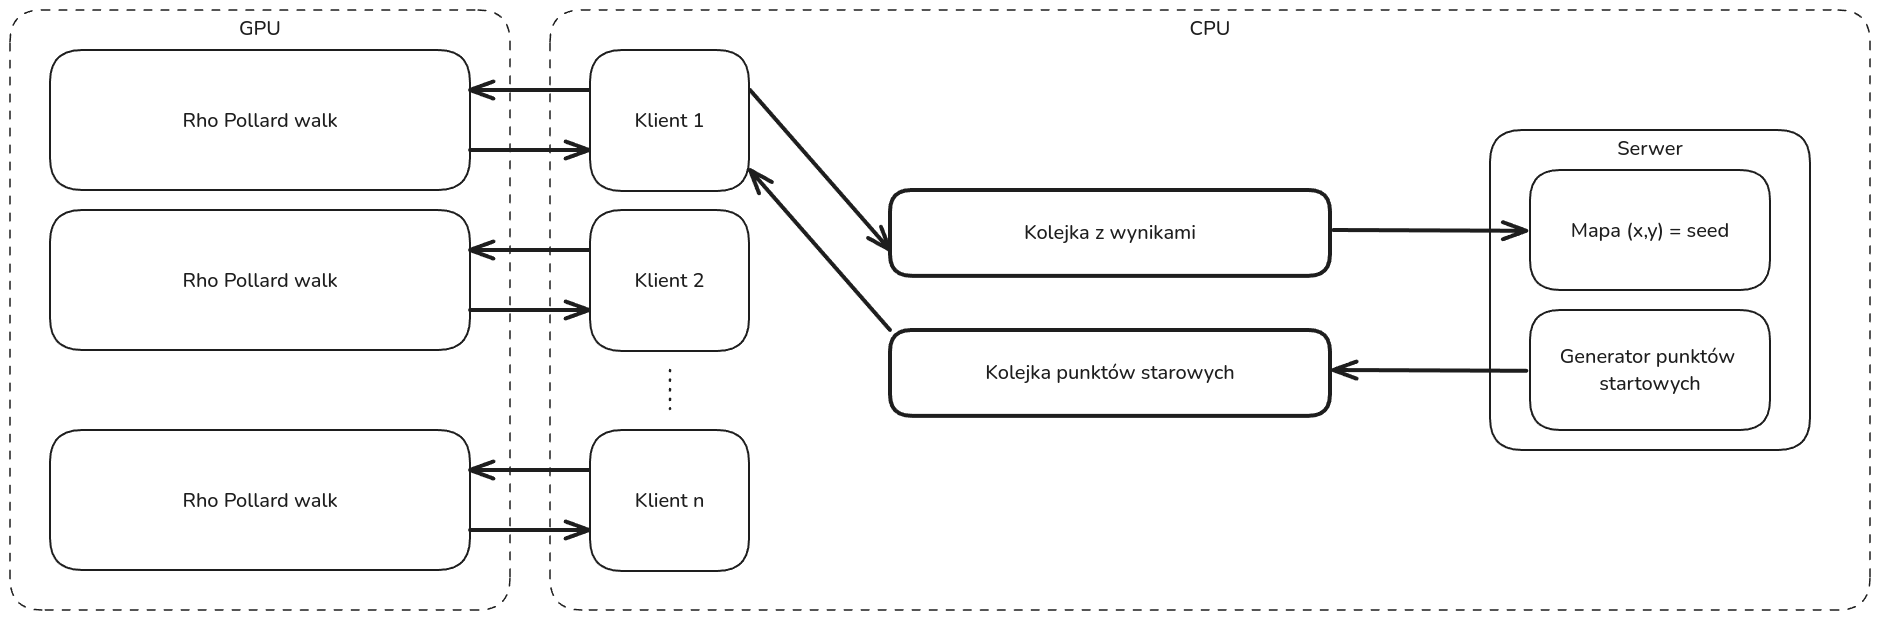
\includegraphics[width=1.1\linewidth]{arch.png}
    \caption{Schemat architektury}
\end{figure}
% \newpage % Zaleca się otwieranie rozdziału od nowej strony.
\section{State~of~Art}
\label{sc:state}

\subsection{GPU}
Procesory graficzne są dedykowane do wykonywania wielu równoległych obliczeń.
Dzięki temu, są bardzo wydajne w zadaniach które można łatwo zrónoleglić.
Wiele algorytmów do kryptoanalizy pozwala na przetwarzanie równoległe, 
w szczególności algorytm \textbf{rho-Pollarda}.
\subsubsection*{Solving Discrete Logarithms in Smooth-Order Groups with CUDA}
W roku 2012 na karcie graficznej NVIDIA Tesla M2050 osiągnięto wydajność na poziomie
51.9 miliona operacji mnożenia modularnego 768-bit na sekundę.
Implementacja opierała się głównie na języku C z CUDA framework wraz z jednostkowymi segmentami
w języku PTX który jest zbiorem instrukcji dla CUDA GPU.
Praca ma dla mnie szczególną na tym etapie, ponieważ razem z pracą udostępniono kod
implementacji na prawach open-source, dodatkowo opisuje
ograniczenia i założenia jakie należy uwzględnić przy implementacji
algorytmu rho-Pollarda na GPU\cite{henry-goldberg-cuda}.

\subsubsection*{ECC2K-130 on NVIDIA GPUs}
Artykuł opisuje implementację algorytmu rho-Pollarda na karcie graficznej NVIDIA 
GTX 295.
Autorzy wybrali krzywą Koblitza ECC2K-130.
Opisano decyzje związane z wyborem bazy ( w tym przypadku wybrano bazę normalną).
Przedstawiono również szczegóły związane z zarządzaniem pamięcią oraz problem związany
z DRAM'em karty (przy pełnej utylizacji GPU w pamięci brakowało miejsca na input)
Wynik: Średnio obliczenie ECDLP na tej krzywej zajełoby 2 lata przy 534 kartach.

\subsection{FPGA}
\subsubsection*{Solving Discrete Logarithms in Smooth-Order Groups with CUDA}
W 2014 opublikowano pracę przedstawiającą implementację FPGA
na platformie Virtex-6.
dedykowaną do rozwiązania logarytmu dyskretnego na 113-bitowej krzywej Koblitza.
Opisano zastosowane zabiegi poprawiające optymalizację, oraz design
poszczególnych moduł
Na przykład w celu lepszej optymalizacji, wykorzystano bazę normalną
$F_{2^m}$ w jednym z modułów do liczenia automorfizmu punktów.
Wynik po ekstrapolacji to 28 dni na rozwiązanie logarytmu na krzywej Koblitza 113 bit.

\subsection{CPU}
CPU nie są najwydajniejszą architekturą do wykonywania równoległych obliczeń.
Zazwyczaj charakteryzują się znacznie wydajniejszymi jednostkami obliczeniowymi (rdzeniami)
niż na przykład GPGPU, ale jest ich również znacznie mnniej niż w GPGPU.
CPUs są najlepiej przystosowane do przetwarzania potokowego.
\subsubsection*{A Review on solving ECDLP over Large Finite Field using Parallel
	Pollard's Rho (p) Method}
Praca przedstawia wyniki czasowe przy obliczaniu ECDLP na
ciele skończonym rzędu p do 85-bitów.
Zastosowano do tego cluster CPU o 256 rdzeniach octa-core.
Artykuł również jest interesujący ponieważ zwięźle opsuje background matematyczny
oraz przejrzyście przedstawia wersję równoległą
algorytmu rho Pollarda\cite{rewiev-elliptic-cpu}.
Wynik to 52 godziny dla krzywej na ciele rozmiaru p = 85-bitów.



\newpage
\section{Implementacja}

\subsection*{Ogólna architektura}

Równoległy algorytm Rho Pollarda zakłada architekturę, w której jeden serwer zbiera wygenerowane przez klientów punkty charakterystyczne i porównuje je
w celu znalezienia kolizji. W mojej pracy rolę serwera pełni program działający na CPU, delegujący obliczenia koprocesora, jakim jest GPU.
Klientami generującym punkty charakerystyczne są instancje funkcji iteracyjnej, uruchamiane na GPU, obliczające kolejne punkty podczas spaceru losowego po krzywej eliptycznej.
W celu uproszczenia implementacji kodu po stronie GPU, oraz utyliacji zasobów serwera w czasie oczekiwania na kolejne serie punktów, punkty startowe
stanowiące punkt wejściowy każdej instancji, generowane są po stronie serwera. Za uruchamianie kolejnych serii obliczeń na koprocesorze, odpowiada program uruchomiony w osobnym wątku
komunikujący się z serwerem za pomocą synchronizowanych kolejek.
Taka implementacja architektury, w której asynchronicznie programy nadzorują pracę GPU, pozwala na bardzo proste rozszerzenie obliczeń o kolejne koprocesory.
Wystarczy uruchomić kolejny wątek z \textit{worker'em} wskazując odpowiedni identyfikator GPU.


\subsection*{Artmetyka na ciele $F_{79}$}

\subsubsection{Biblioteka CGBN}

\subsubsection{Reprezentacja punktów 79 bit na platformie CUDA}
Największym słowem bitowych dostępnym natywnie na platformie CUDA, jest 64 bitowy typ danych. Taka reprezentacja nie wystarcza,
do przeprowadzenia operacji na krzywej ECCp79bit. W tym celu należy przedstawić liczbę większą od natywnego rozmiaru, jako wektor wielu słów bitowych
rozmiaru o jeden mniejszego od największego dostępnego.  Przykładowo, punkt na krzywej eliptycznej o współrzędnych rozmiaru 96 bit, można przedstawić w następujący sposób:

\begin{lstlisting}[language=C++]
typedef struct
{
    uint32_t x[3];
    uint32_t y[3];
} EC_point;
\end{lstlisting}

\subsubsection{Dodawanie}

\subsubsection{Mnożenie}

\subsubsection{Odwrotność modulo p}

\subsection*{Funkcja iterująca}

\subsubsection{Wybór sposobu generowanie kolejnych punktów}

\subsubsection{Wstępnie obliczone punkty}
cytowanie about rho pollard walks

% \subsubsection{Reducja Berreta}

\subsubsection{Obliczanie odwrotnosci w seriach}

\subsection{Tailing effect}
\subsubsection{Rozmiar bloku}
\subsubsection{Uruchomienia asynchroniczne}

\subsection{Serwer}

\subsubsection{GPUWorker}

\subsubsection{Komunikacja}

\section{Wyniki}

\subsection{Dalsze usprawnienia}
Redukcja berreta

\subsection{Porównanie z innymi pracami}

%--------------------------------------------
% Literatura
%--------------------------------------------
\newpage
\printbibliography
%--------------------------------------------
% Spisy (opcjonalne)
%--------------------------------------------
\newpage

% Wykaz symboli i skrótów.
% Pamiętaj, żeby posortować symbole alfabetycznie
% we własnym zakresie. Ponieważ mało kto używa takiego wykazu, 
% uznałem, że robienie automatycznie sortowanej listy
% na poziomie LaTeXa to za duży overkill. 
% Makro \acronymlist generuje właściwy tytuł sekcji, 
% w zależności od języka.
% Makro \acronym dodaje skrót/symbol to listy, 
% zapewniając podstawowe formatowanie.
% //AB
\vspace{0.8cm}
\acronymlist
\acronym{EiTI}{Wydział Elektroniki i Technik Informacyjnych}
\acronym{PW}{Politechnika Warszawska}
\acronym{FPGA}{Field Programmable Gates Array}
\acronym{DLP}{Discrete Logarithm Problem}
\acronym{GF}{Galois Field (ciało skończone)}

\listoffigures              % Spis obrazków. 
\vspace{1cm}                % vertical space
\listoftables               % Spis tabel. 
\vspace{1cm}               % vertical space
\lstlistoflistings 		% Spis wydruków
\vspace{1cm}                % vertical space
\listofappendices           % Spis załączników

% Załączniki

%\newpage
%\appendix{Nazwa załącznika 1}
%\lipsum[1]
%
%\newpage
%\appendix{Nazwa załącznika 2}
%\lipsum[1]
% Załączniki

%\newpage

% jesli sa w~Zalacznikach tabele, rysunki, tak na szybko.. i~wylaczyc \listofappendices
%\section*{Załącznik I. Wykaz komend AT czujnika parkowania AN-101D firmy Shenzhen Winext Technology}
%%\appendix{Wykaz komend AT czujnika parkowania AN-101D firmy Shenzhen Winext Technology.}
%\setcounter{section}{1}
%\renewcommand\thetable{I.\arabic{table}}
%\input{tex/zal-1-komendy-at}
%
%\newpage
%\section*{Załącznik II. Ramki komunikacyjne czujnika parkowania AN-101D firmy Shenzhen Winext Technology}
%%\appendix{Ramki komunikacyjne czujnika parkowania AN-101D firmy Shenzhen Winext Technology.}
%\renewcommand\thefigure{II.\arabic{figure}}
%\input{tex/zal-2-ramki-komunikacyjne}




\end{document} % Dobranoc. 

